\documentclass[tikz,border=2pt]{standalone}
\usepackage{amsmath,amssymb}
\usepackage{pgfplots}
\pgfplotsset{compat=1.18}
\usetikzlibrary{arrows.meta}
\begin{document}
% Makeham force mu_y = A + B c^y with A = 0.001, B = 0.0001, c = 1.1 on a log scale:
% the constant A dominates at young ages, the Gompertz term B c^y (a straight line on the log scale) at old ages;
% mu_40 = 0.001 + 0.0001(1.1)^40 ~ 0.00553.
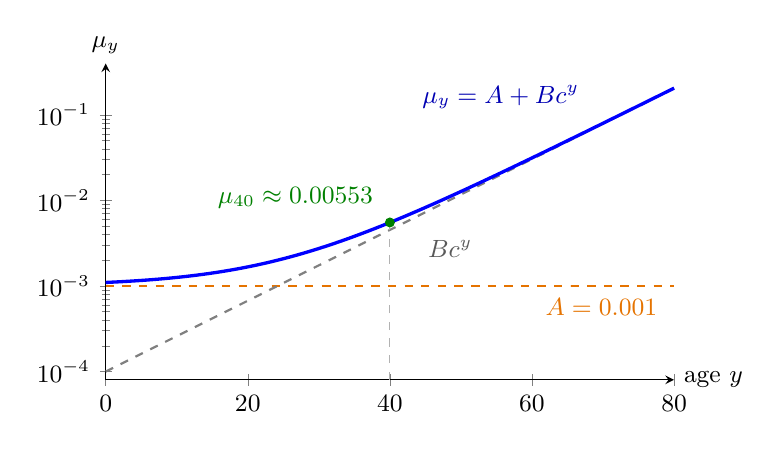
\begin{tikzpicture}[font=\small, >={Latex[length=2mm]}]
  \begin{axis}[
    axis lines=left, xmin=0, xmax=80, ymin=0.00008, ymax=0.4, ymode=log,
    xtick={0,20,40,60,80},
    ytick={0.0001,0.001,0.01,0.1}, yticklabels={$10^{-4}$,$10^{-3}$,$10^{-2}$,$10^{-1}$},
    xlabel={age $y$}, ylabel={$\mu_y$},
    xlabel style={at={(axis description cs:1,0)}, anchor=west},
    ylabel style={rotate=-90, at={(axis description cs:0,1)}, anchor=south},
    samples=100, width=8.8cm, height=5.6cm, clip=false]
    \addplot[orange!90!black, thick, dashed, domain=0:80] {0.001};
    \addplot[gray, thick, dashed, domain=0:80] {0.0001*1.1^x};
    \addplot[blue, very thick, domain=0:80] {0.001+0.0001*1.1^x};
    \draw[gray!60, thin, dashed] (axis cs:40,0.00008) -- (axis cs:40,0.00553);
    \fill[green!50!black] (axis cs:40,0.00553) circle (1.8pt);
    \node[green!50!black, anchor=south east] at (axis cs:39,0.0062) {$\mu_{40}\approx0.00553$};
    \node[orange!90!black, anchor=north east] at (axis cs:79,0.00092) {$A=0.001$};
    \node[gray!70!black, anchor=north west] at (axis cs:44,0.0045) {$Bc^y$};
    \node[blue!70!black, anchor=south east] at (axis cs:68,0.09) {$\mu_y=A+Bc^y$};
  \end{axis}
\end{tikzpicture}
\end{document}
